\documentclass[12pt,a4paper]{article}
\usepackage[utf8]{inputenc}
\usepackage[T1]{fontenc}
\usepackage{geometry}
\usepackage{titlesec}
\usepackage[table]{xcolor}
\usepackage{listings}
\usepackage{graphicx}
\usepackage{fancyhdr}
\usepackage{enumitem}
\usepackage{booktabs}
\usepackage{array}
\usepackage{hyperref}
\usepackage{tikz}
\usetikzlibrary{positioning}
\usepackage{fontawesome5}
\usepackage{lmodern}
\usepackage{parskip}
\usepackage{setspace}
\usepackage{amsmath,amssymb}

% ============================
% DOCUMENT FORMATTING SETTINGS
% ============================
\geometry{a4paper, margin=1in, top=1.2in, bottom=1.2in}
\setlength{\parskip}{0.8em}
\setstretch{1.1}

% ============================
% COLOR DEFINITIONS
% ============================
\definecolor{primary}{RGB}{0, 82, 147}     % Dark blue
\definecolor{secondary}{RGB}{148, 0, 211}  % Purple
\definecolor{accent}{RGB}{220, 53, 69}     % Red
\definecolor{lightgray}{RGB}{245, 245, 245}
\definecolor{darkgray}{RGB}{64, 64, 64}
\definecolor{codegreen}{RGB}{0, 128, 0}
\definecolor{codeblue}{RGB}{0, 0, 255}
\definecolor{codepurple}{RGB}{128, 0, 128}
\definecolor{codegray}{RGB}{128, 128, 128}
\definecolor{backcolour}{RGB}{250, 250, 255}

% ============================
% HEADER AND FOOTER
% ============================
\pagestyle{fancy}
\fancyhf{}
\fancyhead[L]{\small\textcolor{primary}{\textbf{SE3140: System Design and Modeling}}}
\fancyhead[R]{\small\textcolor{darkgray}{\textbf{Design Patterns \& SOLID Principles}}}
\fancyfoot[C]{\thepage}
\renewcommand{\headrulewidth}{0.5pt}
\renewcommand{\headrule}{\hbox to\headwidth{\color{primary}\leaders\hrule height \headrulewidth\hfill}}

% ============================
% TITLE FORMATTING
% ============================
\titleformat{\section}
{\color{primary}\normalfont\Large\bfseries\scshape}
{\thesection}{1em}{}

\titleformat{\subsection}
{\color{secondary}\normalfont\large\bfseries}
{\thesubsection}{1em}{}

\titleformat{\subsubsection}
{\color{accent}\normalfont\normalsize\bfseries}
{\thesubsubsection}{1em}{}

% ============================
% CODE LISTING SETTINGS
% ============================
\lstset{
    backgroundcolor=\color{backcolour},
    commentstyle=\color{codegreen},
    keywordstyle=\color{codeblue},
    numberstyle=\tiny\color{codegray},
    stringstyle=\color{codepurple},
    basicstyle=\ttfamily\footnotesize,
    breakatwhitespace=false,
    breaklines=true,
    captionpos=b,
    keepspaces=true,
    numbers=left,
    numbersep=5pt,
    showspaces=false,
    showstringspaces=false,
    showtabs=false,
    tabsize=2,
    frame=single,
    framerule=0.5pt,
    rulecolor=\color{lightgray},
    title=\lstname
}

% ============================
% CUSTOM COMMANDS
% ============================
\newcommand{\important}[1]{\textbf{\textcolor{accent}{#1}}}
\newcommand{\keyword}[1]{\textbf{\textcolor{codeblue}{#1}}}
\newcommand{\pattern}[1]{\textbf{\textcolor{secondary}{\texttt{#1}}}}
\newcommand{\principle}[1]{\textbf{\textcolor{primary}{#1}}}
\newcommand{\note}[1]{\par\noindent\colorbox{lightgray}{\parbox{\linewidth}{\textit{\textbf{Note:} #1}}}\vspace{0.5em}}

% ============================
% DOCUMENT START
% ============================
\begin{document}

% ============================
% TITLE PAGE
% ============================
\begin{titlepage}
    \centering
    
    % University header
    \begin{tikzpicture}[remember picture, overlay]
        \draw[fill=primary, draw=primary] (current page.north west) rectangle ([yshift=-2.5cm]current page.north east);
    \end{tikzpicture}
    
    \vspace*{.3cm}
    \includegraphics[width=0.3\textwidth]{logo.jpg} % Replace with actual logo
    \vspace{1cm}
    
    {\Huge \color{primary} \textbf{Design Patterns and SOLID Principles}}
    
    \vspace{0.5cm}
    {\Large \color{darkgray} \textbf{Comprehensive Documentation}}
    
    \vspace{1cm}
    
    \begin{minipage}{0.9\textwidth}
        \centering
        \Large
        \textbf{SE3140: System Design and Modeling} \\
        \vspace{0.3cm}
        \textbf{Faculty of Information and Communication Technologies} \\
        \vspace{0.3cm}
        \textbf{Fall 2025} \\
        \vspace{0.3cm}
        \textbf{Lecturer: Engr. Tekoh Palma} \\
        \vspace{0.3cm}
        \textbf{Presentation Date: 7th January 2026}
    \end{minipage}
    
    \vfill
    
    % Group members
    \begin{minipage}{\textwidth}  % Use full width
    \centering  % Changed from \centering
    \large
    \textbf{\color{primary} Group Members} \\
    \vspace{0.6cm}
    \raggedright
    \begin{enumerate}[leftmargin=*, 
    label=\textbf{\arabic*.}, itemsep=0.2cm]
        \item \textbf{Kamdeu Yamdjeuson Neil Marshall [ICTU20241386]}
        \item \textbf{Tuheu Tchoubi Pempem Moussa Fahdil [ICTU20241393]}
        \item \textbf{Kwete Ngnouba Rayan [ICTU2024]}
        \item \textbf{Chijioke Emmanuel Izuchukwu [ICTU2024]}
    \end{enumerate}
\end{minipage}
    
    \begin{tikzpicture}[remember picture, overlay]
        \draw[fill=primary, draw=primary] (current page.south west) rectangle ([yshift=1.5cm]current page.south east);
    \end{tikzpicture}
    
\end{titlepage}

% ============================
% TABLE OF CONTENTS
% ============================
\tableofcontents
\newpage

% ============================
% INTRODUCTION
% ============================
\section{Introduction}
\label{sec:introduction}

\begin{tikzpicture}[remember picture, overlay]
    \node[anchor=north east, xshift=-2cm, yshift=-1.5cm, fill=lightgray, rounded corners, inner sep=5pt, draw=primary, thick] at (current page.north east) {
        \begin{minipage}{0.25\textwidth}
            \footnotesize
            \textbf{\color{primary}Key Concepts:}\\
            • Design Patterns\\
            • SOLID Principles\\
            • Software Architecture\\
            • Maintainability\\
            • Reusability
        \end{minipage}
    };
\end{tikzpicture}

\vspace{1cm}

Software systems inevitably grow in complexity as requirements evolve. Without proper design approaches, software becomes difficult to maintain, extend, and reuse. \important{Design Patterns} and \important{SOLID Principles} provide proven solutions to recurring software design problems and help developers create robust, flexible, and maintainable systems.

This document provides a comprehensive explanation of \pattern{Design Patterns} and \principle{SOLID Principles}. Each design pattern is explained using:
\begin{itemize}[leftmargin=*]
    \item \keyword{Intent} - The purpose of the pattern
    \item \keyword{Motivation} - Why the pattern is needed
    \item \keyword{Structure} - UML or class relationships
    \item \keyword{Code Examples} - Practical implementations
\end{itemize}

Each SOLID principle is demonstrated with \important{clear, well-commented code examples}.

\note{Design patterns are not silver bullets. They should be applied judiciously based on the specific context and requirements of your project.}

% ============================
% DESIGN PATTERNS OVERVIEW
% ============================
\section{Design Patterns Overview}
\label{sec:design-patterns-overview}

\subsection{What Are Design Patterns?}

Design patterns are \important{general reusable solutions} to commonly occurring problems in software design. They are not finished designs that can be directly converted into code; instead, they are \important{templates or guidelines} that describe how to solve a problem in different situations.

\vspace{0.5em}

\begin{table}[h]
    \centering
    \begin{tabular}{|>{\raggedright\arraybackslash}p{0.25\textwidth}|>{\raggedright\arraybackslash}p{0.65\textwidth}|}
        \hline
        \rowcolor{lightgray}
        \textbf{Characteristic} & \textbf{Description} \\
        \hline
        Best Practices & Represent solutions refined over time through collective experience \\
        \hline
        Readability & Improve code readability and maintainability \\
        \hline
        Reusability & Promote reusability and scalability of code \\
        \hline
        Language Independence & Can be implemented in any object-oriented language \\
        \hline
        Problem-Solving & Address specific design problems, not algorithmic problems \\
        \hline
    \end{tabular}
    \caption{Key Characteristics of Design Patterns}
    \label{tab:pattern-characteristics}
\end{table}

\subsection{Difference Between Design Patterns and Algorithms}

\begin{table}[h]
    \centering
    \begin{tabular}{|>{\raggedright\arraybackslash}p{0.2\textwidth}|>{\raggedright\arraybackslash}p{0.35\textwidth}|>{\raggedright\arraybackslash}p{0.35\textwidth}|}
        \hline
        \rowcolor{lightgray}
        \textbf{Aspect} & \textbf{Design Patterns} & \textbf{Algorithms} \\
        \hline
        Purpose & Solve software \important{design} problems & Solve computational \important{processing} problems \\
        \hline
        Level & High-level system design & Low-level step-by-step logic \\
        \hline
        Output & Structure and relationships between classes & A specific result or computation \\
        \hline
        Reusability & Conceptual and architectural & Code-oriented and mathematical \\
        \hline
        Example & \pattern{Singleton}, \pattern{Factory}, \pattern{Observer} & Sorting, Searching, Graph traversal \\
        \hline
    \end{tabular}
    \caption{Design Patterns vs. Algorithms}
    \label{tab:patterns-vs-algorithms}
\end{table}

\subsection{Types of Design Patterns}

Design patterns are classified into three main categories:

\begin{figure}[h]
    \centering
    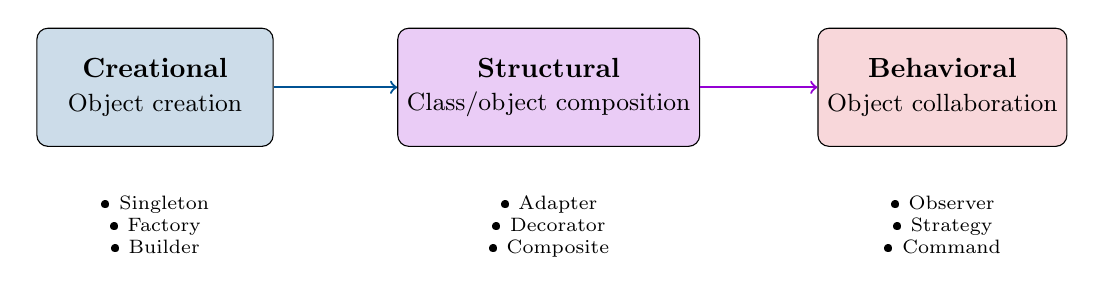
\begin{tikzpicture}
        \node[draw, fill=primary!20, rounded corners, minimum width=3cm, minimum height=1.5cm, align=center] (creational) at (0,0) {\textbf{Creational}\\\small{Object creation}};
        \node[draw, fill=secondary!20, rounded corners, minimum width=3cm, minimum height=1.5cm, align=center] (structural) at (5,0) {\textbf{Structural}\\\small{Class/object composition}};
        \node[draw, fill=accent!20, rounded corners, minimum width=3cm, minimum height=1.5cm, align=center] (behavioral) at (10,0) {\textbf{Behavioral}\\\small{Object collaboration}};
        
        \draw[->, thick, primary] (creational.east) -- (structural.west);
        \draw[->, thick, secondary] (structural.east) -- (behavioral.west);
        
        \node[below=0.5cm of creational, text width=3cm, align=center, font=\scriptsize] {\textbullet\ Singleton\\\textbullet\ Factory\\\textbullet\ Builder};

\node[below=0.5cm of structural, text width=3cm, align=center, font=\scriptsize] {\textbullet\ Adapter\\\textbullet\ Decorator\\\textbullet\ Composite};

\node[below=0.5cm of behavioral, text width=3cm, align=center, font=\scriptsize] {\textbullet\ Observer\\\textbullet\ Strategy\\\textbullet\ Command};

    \end{tikzpicture}
    \caption{Three Categories of Design Patterns}
    \label{fig:pattern-categories}
\end{figure}

% ============================
% CREATIONAL DESIGN PATTERNS
% ============================
\section{Creational Design Patterns}
\label{sec:creational-patterns}

Creational patterns abstract the instantiation process. They help make a system independent of how its objects are created, composed, and represented.

\subsection{Singleton Pattern}
\label{subsec:singleton}

\begin{tabular}{p{0.9\textwidth}}
    \hline
    \rowcolor{lightgray}
    \textbf{Intent:} Ensure a class has only one instance and provide a global point of access to it. \\
    \hline
    \textbf{Motivation:} Singleton is useful when exactly one object is needed to coordinate actions across the system (e.g., configuration manager, logging service). \\
    \hline
    \textbf{Structure:} \textbf{Private} static instance, \textbf{private} constructor, \textbf{public} static access method. \\
    \hline
\end{tabular}

\vspace{1em}

\begin{lstlisting}[language=C++, caption={Singleton Pattern Implementation in C++}, label=lst:singleton]
#include <iostream>

class Singleton {
private:
    // 1. Private static instance
    static Singleton* instance;
    
    // 2. Private constructor
    Singleton() {
        std::cout << "Singleton instance created." << std::endl;
    }
    
    // Prevent copying
    Singleton(const Singleton&) = delete;
    Singleton& operator=(const Singleton&) = delete;

public:
    // 3. Public static access method
    static Singleton* getInstance() {
        if (instance == nullptr) {
            instance = new Singleton();
        }
        return instance;
    }
    
    void doSomething() {
        std::cout << "Singleton is doing something." << std::endl;
    }
};

// Initialize static member
Singleton* Singleton::instance = nullptr;

// Usage example
int main() {
    // Get the singleton instance
    Singleton* s1 = Singleton::getInstance();
    s1->doSomething();
    
    // This will return the same instance
    Singleton* s2 = Singleton::getInstance();
    
    // s1 and s2 are the same instance
    std::cout << "Are they same? " << (s1 == s2 ? "Yes" : "No") << std::endl;
    
    return 0;
}
\end{lstlisting}

\subsection{Factory Method Pattern}
\label{subsec:factory-method}

\begin{tabular}{p{0.9\textwidth}}
    \hline
    \rowcolor{lightgray}
    \textbf{Intent:} Define an interface for creating objects but allow subclasses to alter the type of objects created. \\
    \hline
    \textbf{Motivation:} Factory Method promotes loose coupling by eliminating the need to bind application-specific classes into the code. \\
    \hline
    \textbf{Structure:} Product interface → ConcreteProduct → Creator (factory) class. \\
    \hline
\end{tabular}

\vspace{1em}

\begin{lstlisting}[language=Java, caption={Factory Method Pattern Implementation in Java}, label=lst:factory-method]
// Product interface
interface Shape {
    void draw();
}

// Concrete Products
class Circle implements Shape {
    @Override
    public void draw() {
        System.out.println("Drawing a Circle");
    }
}

class Rectangle implements Shape {
    @Override
    public void draw() {
        System.out.println("Drawing a Rectangle");
    }
}

class Square implements Shape {
    @Override
    public void draw() {
        System.out.println("Drawing a Square");
    }
}

// Creator (Factory) class
class ShapeFactory {
    // Factory method
    public Shape getShape(String shapeType) {
        if (shapeType == null) {
            return null;
        }
        
        if (shapeType.equalsIgnoreCase("CIRCLE")) {
            return new Circle();
        } else if (shapeType.equalsIgnoreCase("RECTANGLE")) {
            return new Rectangle();
        } else if (shapeType.equalsIgnoreCase("SQUARE")) {
            return new Square();
        }
        
        return null;
    }
}

// Client code
public class FactoryPatternDemo {
    public static void main(String[] args) {
        ShapeFactory shapeFactory = new ShapeFactory();
        
        // Get objects without knowing the concrete classes
        Shape shape1 = shapeFactory.getShape("CIRCLE");
        shape1.draw();
        
        Shape shape2 = shapeFactory.getShape("RECTANGLE");
        shape2.draw();
        
        Shape shape3 = shapeFactory.getShape("SQUARE");
        shape3.draw();
    }
}
\end{lstlisting}

% ============================
% STRUCTURAL DESIGN PATTERNS
% ============================
\section{Structural Design Patterns}
\label{sec:structural-patterns}

Structural patterns are concerned with how classes and objects are composed to form larger structures.

\subsection{Adapter Pattern}
\label{subsec:adapter}

\begin{tabular}{p{0.9\textwidth}}
    \hline
    \rowcolor{lightgray}
    \textbf{Intent:} Convert the interface of a class into another interface that clients expect. \\
    \hline
    \textbf{Motivation:} Adapter allows reuse of existing classes whose interfaces do not match the system requirements. \\
    \hline
    \textbf{Structure:} Target interface ← Adapter ← Adaptee. \\
    \hline
\end{tabular}

\vspace{1em}

\begin{lstlisting}[language=C++, caption={Adapter Pattern Implementation in C++}, label=lst:adapter]
#include <iostream>
#include <string>

// Legacy class with incompatible interface
class LegacyRectangle {
private:
    int x1, y1, x2, y2;
    
public:
    LegacyRectangle(int x1, int y1, int x2, int y2) 
        : x1(x1), y1(y1), x2(x2), y2(y2) {
        std::cout << "LegacyRectangle: " << x1 << "," << y1 
                  << " to " << x2 << "," << y2 << std::endl;
    }
    
    void oldDraw() {
        std::cout << "LegacyRectangle: oldDraw()." << std::endl;
    }
};

// New interface expected by client
class Rectangle {
public:
    virtual void draw(int x, int y, int width, int height) = 0;
    virtual ~Rectangle() {}
};

// Adapter class
class RectangleAdapter : public Rectangle {
private:
    LegacyRectangle* legacyRect;
    
public:
    RectangleAdapter(LegacyRectangle* rect) : legacyRect(rect) {}
    
    void draw(int x, int y, int width, int height) override {
        // Convert new interface to legacy interface
        int x2 = x + width;
        int y2 = y + height;
        
        // Create legacy rectangle with converted parameters
        LegacyRectangle adaptedRect(x, y, x2, y2);
        adaptedRect.oldDraw();
        
        std::cout << "Adapter: Translated new interface to legacy." << std::endl;
    }
};

// Client code
int main() {
    LegacyRectangle* legacy = new LegacyRectangle(0, 0, 20, 30);
    
    // Using adapter to make legacy compatible with new interface
    Rectangle* adapter = new RectangleAdapter(legacy);
    adapter->draw(5, 10, 50, 60);  // Uses new interface
    
    delete legacy;
    delete adapter;
    
    return 0;
}
\end{lstlisting}

\subsection{Decorator Pattern}
\label{subsec:decorator}

\begin{tabular}{p{0.9\textwidth}}
    \hline
    \rowcolor{lightgray}
    \textbf{Intent:} Attach additional responsibilities to an object dynamically. \\
    \hline
    \textbf{Motivation:} Decorator provides a flexible alternative to subclassing for extending functionality. \\
    \hline
    \textbf{Structure:} Component interface → ConcreteComponent → Decorator → ConcreteDecorator. \\
    \hline
\end{tabular}

\vspace{1em}

\begin{lstlisting}[language=C++, caption={Decorator Pattern Implementation in C++}, label=lst:decorator]
#include <iostream>
#include <string>

// Component interface
class Coffee {
public:
    virtual std::string getDescription() const = 0;
    virtual double cost() const = 0;
    virtual ~Coffee() {}
};

// Concrete Component
class SimpleCoffee : public Coffee {
public:
    std::string getDescription() const override {
        return "Simple Coffee";
    }
    
    double cost() const override {
        return 2.0;
    }
};

// Decorator base class
class CoffeeDecorator : public Coffee {
protected:
    Coffee* coffee;
    
public:
    CoffeeDecorator(Coffee* c) : coffee(c) {}
    
    std::string getDescription() const override {
        return coffee->getDescription();
    }
    
    double cost() const override {
        return coffee->cost();
    }
};

// Concrete Decorators
class MilkDecorator : public CoffeeDecorator {
public:
    MilkDecorator(Coffee* c) : CoffeeDecorator(c) {}
    
    std::string getDescription() const override {
        return coffee->getDescription() + ", Milk";
    }
    
    double cost() const override {
        return coffee->cost() + 0.5;
    }
};

class SugarDecorator : public CoffeeDecorator {
public:
    SugarDecorator(Coffee* c) : CoffeeDecorator(c) {}
    
    std::string getDescription() const override {
        return coffee->getDescription() + ", Sugar";
    }
    
    double cost() const override {
        return coffee->cost() + 0.2;
    }
};

// Client code
int main() {
    // Start with simple coffee
    Coffee* coffee = new SimpleCoffee();
    std::cout << "Order: " << coffee->getDescription() 
              << " Cost: $" << coffee->cost() << std::endl;
    
    // Add milk
    coffee = new MilkDecorator(coffee);
    std::cout << "Order: " << coffee->getDescription() 
              << " Cost: $" << coffee->cost() << std::endl;
    
    // Add sugar
    coffee = new SugarDecorator(coffee);
    std::cout << "Final Order: " << coffee->getDescription() 
              << " Cost: $" << coffee->cost() << std::endl;
    
    delete coffee;
    return 0;
}
\end{lstlisting}

% ============================
% BEHAVIORAL DESIGN PATTERNS
% ============================
\section{Behavioral Design Patterns}
\label{sec:behavioral-patterns}

Behavioral patterns are concerned with algorithms and the assignment of responsibilities between objects.

\subsection{Observer Pattern}
\label{subsec:observer}

\begin{tabular}{p{0.9\textwidth}}
    \hline
    \rowcolor{lightgray}
    \textbf{Intent:} Define a one-to-many dependency so that when one object changes state, all its dependents are notified automatically. \\
    \hline
    \textbf{Motivation:} Useful in event-driven systems where multiple components must react to changes in another component without being tightly coupled. \\
    \hline
    \textbf{Structure:} Subject interface $\rightarrow$ ConcreteSubject $\leftrightarrow$ Observer interface $\rightarrow$ ConcreteObserver. \\
    \hline
\end{tabular}

\vspace{1em}

\begin{lstlisting}[language=C++, caption={Observer Pattern Implementation in C++}, label=lst:observer]
#include <iostream>
#include <vector>
#include <string>
#include <algorithm>

// Forward declaration
class Observer;

// Subject interface
class Subject {
public:
    virtual void attach(Observer* observer) = 0;
    virtual void detach(Observer* observer) = 0;
    virtual void notify() = 0;
    virtual ~Subject() {}
};

// Observer interface
class Observer {
public:
    virtual void update(const std::string& message) = 0;
    virtual ~Observer() {}
};

// Concrete Subject
class NewsPublisher : public Subject {
private:
    std::vector<Observer*> observers;
    std::string latestNews;
    
public:
    void attach(Observer* observer) override {
        observers.push_back(observer);
        std::cout << "Observer attached." << std::endl;
    }
    
    void detach(Observer* observer) override {
        observers.erase(std::remove(observers.begin(), observers.end(), observer), 
                       observers.end());
        std::cout << "Observer detached." << std::endl;
    }
    
    void notify() override {
        std::cout << "Notifying " << observers.size() << " observers..." << std::endl;
        for (Observer* observer : observers) {
            observer->update(latestNews);
        }
    }
    
    void publishNews(const std::string& news) {
        latestNews = news;
        std::cout << "\n=== Publishing News: " << news << " ===" << std::endl;
        notify();
    }
};

// Concrete Observer
class NewsSubscriber : public Observer {
private:
    std::string name;
    
public:
    NewsSubscriber(const std::string& name) : name(name) {}
    
    void update(const std::string& message) override {
        std::cout << "Subscriber [" << name << "] received: " << message << std::endl;
    }
};

// Client code
int main() {
    // Create publisher
    NewsPublisher publisher;
    
    // Create subscribers
    NewsSubscriber subscriber1("Alice");
    NewsSubscriber subscriber2("Bob");
    NewsSubscriber subscriber3("Charlie");
    
    // Attach subscribers
    publisher.attach(&subscriber1);
    publisher.attach(&subscriber2);
    publisher.attach(&subscriber3);
    
    // Publish news (observers get notified)
    publisher.publishNews("Breaking: New Design Pattern Course Available!");
    publisher.publishNews("Update: SOLID Principles Workshop Tomorrow");
    
    // Detach one subscriber
    publisher.detach(&subscriber2);
    
    // Publish more news
    publisher.publishNews("Reminder: Project Submission Deadline Extended");
    
    return 0;
}
\end{lstlisting}

% ============================
% SOLID PRINCIPLES
% ============================
\section{SOLID Principles}
\label{sec:solid-principles}

The SOLID principles are five design principles that help create maintainable, understandable, and flexible software. They were introduced by Robert C. Martin (Uncle Bob).

\vspace{1em}

\begin{table}[h]
    \centering
    \begin{tabular}{|>{\raggedright\arraybackslash}p{0.15\textwidth}|>{\raggedright\arraybackslash}p{0.25\textwidth}|>{\raggedright\arraybackslash}p{0.5\textwidth}|}
        \hline
        \rowcolor{lightgray}
        \textbf{Letter} & \textbf{Principle} & \textbf{Core Idea} \\
        \hline
        \principle{S} & Single Responsibility & A class should have only one reason to change \\
        \hline
        \principle{O} & Open/Closed & Software entities should be open for extension but closed for modification \\
        \hline
        \principle{L} & Liskov Substitution & Objects of a superclass should be replaceable with objects of a subclass \\
        \hline
        \principle{I} & Interface Segregation & Clients should not be forced to depend on interfaces they don't use \\
        \hline
        \principle{D} & Dependency Inversion & Depend on abstractions, not on concretions \\
        \hline
    \end{tabular}
    \caption{SOLID Principles Overview}
    \label{tab:solid-overview}
\end{table}

\subsection{Single Responsibility Principle (SRP)}
\label{subsec:srp}

\important{Definition:} A class should have only one reason to change, meaning it should have only one job or responsibility.

\begin{lstlisting}[language=C++, caption={Single Responsibility Principle Example}, label=lst:srp]
#include <iostream>
#include <string>
#include <fstream>

// BAD DESIGN: Class with multiple responsibilities
class EmployeeBad {
private:
    std::string name;
    std::string position;
    double salary;
    
public:
    EmployeeBad(const std::string& n, const std::string& p, double s)
        : name(n), position(p), salary(s) {}
    
    // Responsibility 1: Employee data management
    void setSalary(double s) { salary = s; }
    double getSalary() const { return salary; }
    
    // Responsibility 2: Report generation (should be separate)
    void generateReport() {
        std::cout << "Report for " << name << std::endl;
        std::cout << "Position: " << position << std::endl;
        std::cout << "Salary: $" << salary << std::endl;
    }
    
    // Responsibility 3: Data persistence (should be separate)
    void saveToFile(const std::string& filename) {
        std::ofstream file(filename);
        file << name << "," << position << "," << salary;
        file.close();
    }
};

// GOOD DESIGN: Separated responsibilities
class Employee {
private:
    std::string name;
    std::string position;
    double salary;
    
public:
    Employee(const std::string& n, const std::string& p, double s)
        : name(n), position(p), salary(s) {}
    
    // Only employee-related methods
    void setSalary(double s) { salary = s; }
    double getSalary() const { return salary; }
    std::string getName() const { return name; }
    std::string getPosition() const { return position; }
};

// Separate class for report generation
class ReportGenerator {
public:
    static void generateEmployeeReport(const Employee& emp) {
        std::cout << "\n=== Employee Report ===" << std::endl;
        std::cout << "Name: " << emp.getName() << std::endl;
        std::cout << "Position: " << emp.getPosition() << std::endl;
        std::cout << "Salary: $" << emp.getSalary() << std::endl;
        std::cout << "=======================" << std::endl;
    }
};

// Separate class for data persistence
class EmployeeRepository {
public:
    static void saveToFile(const Employee& emp, const std::string& filename) {
        std::ofstream file(filename);
        file << emp.getName() << "," << emp.getPosition() << "," << emp.getSalary();
        file.close();
        std::cout << "Employee data saved to " << filename << std::endl;
    }
    
    static Employee loadFromFile(const std::string& filename) {
        std::ifstream file(filename);
        std::string name, position;
        double salary;
        
        std::getline(file, name, ',');
        std::getline(file, position, ',');
        file >> salary;
        
        return Employee(name, position, salary);
    }
};

// Client code demonstrating SRP
int main() {
    // Create employee
    Employee emp("John Doe", "Software Engineer", 75000.0);
    
    // Generate report using separate class
    ReportGenerator::generateEmployeeReport(emp);
    
    // Save data using separate class
    EmployeeRepository::saveToFile(emp, "employee_data.txt");
    
    // Load data using separate class
    Employee loadedEmp = EmployeeRepository::loadFromFile("employee_data.txt");
    ReportGenerator::generateEmployeeReport(loadedEmp);
    
    return 0;
}
\end{lstlisting}

\subsection{Open/Closed Principle (OCP)}
\label{subsec:ocp}

\important{Definition:} Software entities (classes, modules, functions) should be open for extension but closed for modification.

\begin{lstlisting}[language=C++, caption={Open/Closed Principle Example}, label=lst:ocp]
#include <iostream>
#include <vector>
#include <memory>

// BAD DESIGN: Not following OCP
class ShapeBad {
    // Type field to distinguish shapes
    enum Type { CIRCLE, SQUARE, TRIANGLE } type;
    
    // For circle
    double radius;
    
    // For square
    double side;
    
    // For triangle
    double base, height;
    
public:
    ShapeBad(Type t, double r) : type(t), radius(r) {} // Circle
    ShapeBad(Type t, double s) : type(t), side(s) {}    // Square
    ShapeBad(Type t, double b, double h) : type(t), base(b), height(h) {} // Triangle
    
    double area() const {
        switch (type) {
            case CIRCLE: return 3.14159 * radius * radius;
            case SQUARE: return side * side;
            case TRIANGLE: return 0.5 * base * height;
            default: return 0;
        }
    }
    // Problem: Adding new shape requires modifying this class
};

// GOOD DESIGN: Following OCP
class Shape {
public:
    virtual double area() const = 0;
    virtual ~Shape() {}
};

class Circle : public Shape {
private:
    double radius;
    
public:
    Circle(double r) : radius(r) {}
    
    double area() const override {
        return 3.14159 * radius * radius;
    }
};

class Square : public Shape {
private:
    double side;
    
public:
    Square(double s) : side(s) {}
    
    double area() const override {
        return side * side;
    }
};

class Triangle : public Shape {
private:
    double base, height;
    
public:
    Triangle(double b, double h) : base(b), height(h) {}
    
    double area() const override {
        return 0.5 * base * height;
    }
};

// NEW SHAPE: Can be added without modifying existing code
class Rectangle : public Shape {
private:
    double width, height;
    
public:
    Rectangle(double w, double h) : width(w), height(h) {}
    
    double area() const override {
        return width * height;
    }
};

// AreaCalculator is closed for modification but open for extension
class AreaCalculator {
public:
    static double totalArea(const std::vector<std::shared_ptr<Shape>>& shapes) {
        double total = 0;
        for (const auto& shape : shapes) {
            total += shape->area();
        }
        return total;
    }
};

// Client code demonstrating OCP
int main() {
    std::vector<std::shared_ptr<Shape>> shapes;
    
    // Add various shapes
    shapes.push_back(std::make_shared<Circle>(5.0));
    shapes.push_back(std::make_shared<Square>(4.0));
    shapes.push_back(std::make_shared<Triangle>(3.0, 6.0));
    
    // New shape added without modifying AreaCalculator
    shapes.push_back(std::make_shared<Rectangle>(4.0, 6.0));
    
    // Calculate total area
    double total = AreaCalculator::totalArea(shapes);
    std::cout << "Total area of all shapes: " << total << std::endl;
    
    return 0;
}
\end{lstlisting}

\subsection{Liskov Substitution Principle (LSP)}
\label{subsec:lsp}

\important{Definition:} Objects of a superclass should be replaceable with objects of a subclass without affecting the correctness of the program.

\begin{lstlisting}[language=C++, caption={Liskov Substitution Principle Example}, label=lst:lsp]
#include <iostream>
#include <vector>
#include <memory>

// BAD DESIGN: Violating LSP
class RectangleBad {
protected:
    double width, height;
    
public:
    RectangleBad(double w, double h) : width(w), height(h) {}
    
    virtual void setWidth(double w) { width = w; }
    virtual void setHeight(double h) { height = h; }
    
    double getWidth() const { return width; }
    double getHeight() const { return height; }
    
    double area() const { return width * height; }
};

class SquareBad : public RectangleBad {
public:
    SquareBad(double side) : RectangleBad(side, side) {}
    
    void setWidth(double w) override {
        width = w;
        height = w; // Violates LSP: Changes height too
    }
    
    void setHeight(double h) override {
        height = h;
        width = h; // Violates LSP: Changes width too
    }
};

// Problematic usage
void testRectangleBad(RectangleBad& rect) {
    rect.setWidth(5);
    rect.setHeight(4);
    std::cout << "Expected area: 20, Actual area: " << rect.area() << std::endl;
    // For SquareBad, this prints 16, not 20!
}

// GOOD DESIGN: Following LSP
class ShapeLSP {
public:
    virtual double area() const = 0;
    virtual ~ShapeLSP() {}
};

class RectangleLSP : public ShapeLSP {
protected:
    double width, height;
    
public:
    RectangleLSP(double w, double h) : width(w), height(h) {}
    
    virtual void setWidth(double w) { width = w; }
    virtual void setHeight(double h) { height = h; }
    
    double getWidth() const { return width; }
    double getHeight() const { return height; }
    
    double area() const override { return width * height; }
};

class SquareLSP : public ShapeLSP {
private:
    double side;
    
public:
    SquareLSP(double s) : side(s) {}
    
    void setSide(double s) { side = s; }
    double getSide() const { return side; }
    
    double area() const override { return side * side; }
};

// Factory functions to create shapes
std::shared_ptr<RectangleLSP> createRectangle(double width, double height) {
    return std::make_shared<RectangleLSP>(width, height);
}

std::shared_ptr<SquareLSP> createSquare(double side) {
    return std::make_shared<SquareLSP>(side);
}

// Client code demonstrating LSP
int main() {
    std::vector<std::shared_ptr<ShapeLSP>> shapes;
    
    // Add different shapes
    shapes.push_back(createRectangle(5, 4));
    shapes.push_back(createSquare(5));
    
    // Calculate total area
    double totalArea = 0;
    for (const auto& shape : shapes) {
        totalArea += shape->area();
        std::cout << "Shape area: " << shape->area() << std::endl;
    }
    
    std::cout << "\nTotal area: " << totalArea << std::endl;
    
    // Demonstrate that each shape maintains its own invariants
    auto rect = createRectangle(10, 5);
    std::cout << "\nRectangle area: " << rect->area() << std::endl;
    
    auto square = createSquare(10);
    std::cout << "Square area: " << square->area() << std::endl;
    
    return 0;
}
\end{lstlisting}

% ============================
% CONCLUSION
% ============================
\section{Conclusion}
\label{sec:conclusion}

Design Patterns and SOLID Principles are essential tools for professional software development. When applied correctly, they lead to systems that are easier to understand, maintain, test, and extend.

\begin{figure}[h]
    \centering
    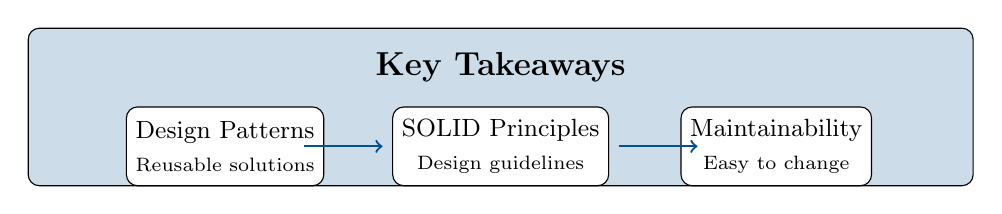
\begin{tikzpicture}
        \draw[fill=primary!20, rounded corners] (0,0) rectangle (12,2);
        \node at (6,1.5) {\textbf{\large Key Takeaways}};
        
        \node[draw, fill=white, rounded corners, minimum height=1cm, align=center] at (2.5,0.5) {\small Design Patterns\\\scriptsize Reusable solutions};
        \node[draw, fill=white, rounded corners, minimum height=1cm, align=center] at (6,0.5) {\small SOLID Principles\\\scriptsize Design guidelines};
        \node[draw, fill=white, rounded corners, minimum height=1cm, align=center] at (9.5,0.5) {\small Maintainability\\\scriptsize Easy to change};
        
        \draw[->, thick, primary] (3.5,0.5) -- (4.5,0.5);
        \draw[->, thick, primary] (7.5,0.5) -- (8.5,0.5);
    \end{tikzpicture}
    \caption{Design Patterns and SOLID Principles Synergy}
    \label{fig:conclusion}
\end{figure}

\vspace{1em}

\begin{itemize}
    \item \important{Design Patterns} provide \textbf{templates} for solving common problems
    \item \important{SOLID Principles} provide \textbf{guidelines} for creating maintainable code
    \item Together, they form a \textbf{powerful toolkit} for software architects and developers
    \item Proper application leads to \textbf{reduced technical debt} and \textbf{easier maintenance}
\end{itemize}

\note{Remember that patterns and principles should be applied thoughtfully, not dogmatically. The goal is to create software that is easy to change and maintain, not to use every pattern possible.}

\vspace{1em}

\noindent\textbf{\color{primary}FURTHER READING:}
\begin{itemize}
    \item Gamma, E., et al. (1994). \textit{Design Patterns: Elements of Reusable Object-Oriented Software}
    \item Martin, R. C. (2002). \textit{Agile Software Development: Principles, Patterns, and Practices}
    \item Freeman, E., et al. (2004). \textit{Head First Design Patterns}
\end{itemize}

\end{document}